\subsection{Dominion}\label{dominion}
De 'Dominion' module wordt gebruikt voor het aanmaken van subsites. Ga naar \drupalpath{admin/structure/dominion} voor een overzicht van alle subsites. 


\bigskip

\begin{center}
	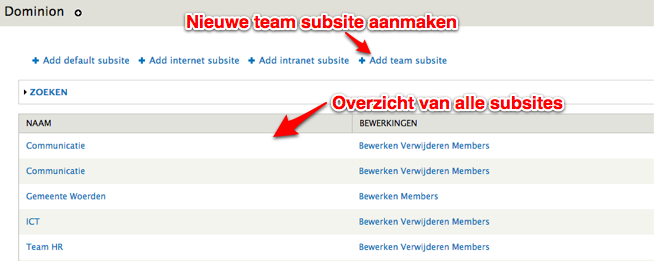
\includegraphics[width=\textwidth]{img/dominion1.png}
\end{center}


\subsubsection{Team subsite toevoegen}\label{teamsubsitetoevoegen}
Klik op 'Add team subsite' om een nieuwe team subsite toe te voegen. 

\begin{enumerate}
\item Vul bij het veld 'Naam' een naam in voor de subsite.
\item Kies bij 'Domain type' voor 'Use a directory'.
\item Kies bij 'Domein' voor 'intranet.dimpact.nl'
\item Vul bij het veld 'Map' de map in voor de subsite
\item Specificeer eventueel de overige opties
\item Klik op de knop 'Opslaan' om de subsite toe te voegen 
\end{enumerate}

\bigskip

\begin{center}
	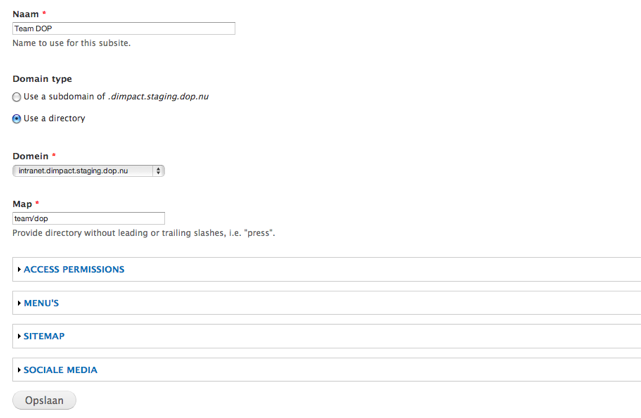
\includegraphics[width=\textwidth]{img/dominion2.png}
\end{center}

\subsubsection{Team members beheren}\label{teammembersbeheren}
Aan elke subsite kunnen 'Members' worden toegevoegd.

\bigskip

Klik op 'Members' bij de betreffende subsite om 'Members' toe te voegen.

\begin{center}
	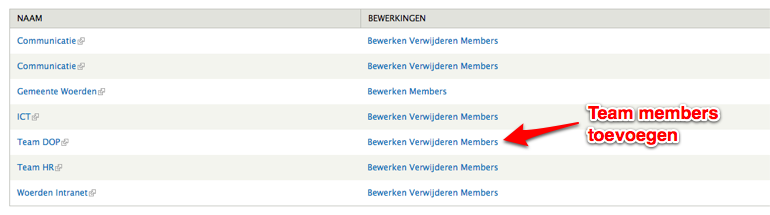
\includegraphics[width=\textwidth]{img/dominion3.png}
\end{center}

\bigskip

Vul de gebruikersnaam of e-mail adres in, selecteer eventueel een domein specifieke rol en klik vervolgens op de knop 'Toevoegen' om de gebruiker toe te voegen aan de lijst van 'Members'.

\bigskip

\begin{center}
	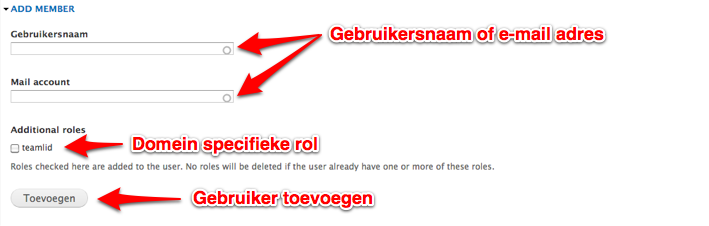
\includegraphics[width=\textwidth]{img/dominion4.png}
\end{center}
